\documentclass[10pt,a4paper]{article}
\usepackage{hyperref}
\usepackage{listings}
\usepackage[cm]{fullpage}
\usepackage{graphicx}
\usepackage{placeins}


\title{IDAPI Coursework Part 4 - Principal Component Analysis}
\author{Sebastian Grubb \href{mailto:sg3510@ic.ac.uk}{sg3510@ic.ac.uk}\\Michael Murray \href{mailto:mm5110@ic.ac.uk}{mm5110@ic.ac.uk}}
\date{\today}



\begin{document}
\maketitle


\section{Results}
\begin{verbatim}
Coursework Four Results by sg3510 and mm5110

Mean vector Hepatitis C:
 1.164  3.916  0.448  5.679  4.865  3.778  4.127  3.604  0.217 

Covariance matrix of the Hepatitis C:
 5.880  0.245 -0.004 -0.284 -0.346 -0.417 -0.481 -0.267 -0.067 
 0.245  7.572  0.073 -0.358 -0.346  0.257  2.273  0.946 -0.032 
-0.004  0.073  0.247 -0.116 -0.039 -0.003  0.100  0.066 -0.005 
-0.284 -0.358 -0.116 16.960  7.969  4.443 -1.036 -0.306  0.047 
-0.346 -0.346 -0.039  7.969  8.361  4.921 -0.763 -0.752 -0.001 
-0.417  0.257 -0.003  4.443  4.921  6.683 -0.087 -0.376 -0.141 
-0.481  2.273  0.100 -1.036 -0.763 -0.087 20.583  1.122  0.014 
-0.267  0.946  0.066 -0.306 -0.752 -0.376  1.122  4.317  0.119 
-0.067 -0.032 -0.005  0.047 -0.001 -0.141  0.014  0.119  0.170 

Component magnitudes:
1206.254 -1590.133 -248.136 -821.249 246.009 -771.900 963.633 376.967 161.599 -533.276 
\end{verbatim}
\FloatBarrier
\newpage
\section{Eigenface images from 4.3}
\begin{figure}[h!]
  \caption{Images of all 10 eigenfaces}
  \centering
  
  \begin{tabular}{ c c c }
    0. 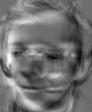
\includegraphics[width=0.25\textwidth]{PrincipalComponent0.jpg} & 1. 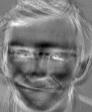
\includegraphics[width=0.25\textwidth]{PrincipalComponent1.jpg} & 2. 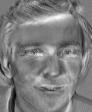
\includegraphics[width=0.25\textwidth]{PrincipalComponent2.jpg} \\
    3. 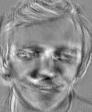
\includegraphics[width=0.25\textwidth]{PrincipalComponent3.jpg} & 4. 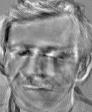
\includegraphics[width=0.25\textwidth]{PrincipalComponent4.jpg} & 5. 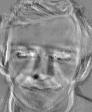
\includegraphics[width=0.25\textwidth]{PrincipalComponent5.jpg} \\
    6. 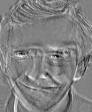
\includegraphics[width=0.25\textwidth]{PrincipalComponent6.jpg} & 7. 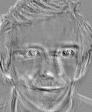
\includegraphics[width=0.25\textwidth]{PrincipalComponent7.jpg} & 8. 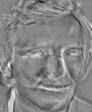
\includegraphics[width=0.25\textwidth]{PrincipalComponent8.jpg} \\
    9. 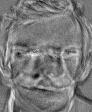
\includegraphics[width=0.25\textwidth]{PrincipalComponent9.jpg}
  \end{tabular}
\end{figure}
\FloatBarrier
\section{Partial Reconstructions from 4.4}
\begin{figure}[h!]
  \caption{Images of all 10 partial reconstructions, including mean}
  \centering
  
  \begin{tabular}{ c c c }
    0. 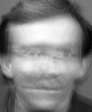
\includegraphics[width=0.25\textwidth]{PartialReconstruction0.jpg} & 1. 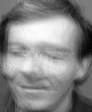
\includegraphics[width=0.25\textwidth]{PartialReconstruction1.jpg} & 2. 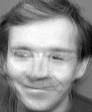
\includegraphics[width=0.25\textwidth]{PartialReconstruction2.jpg} \\
    3. 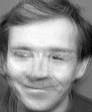
\includegraphics[width=0.25\textwidth]{PartialReconstruction3.jpg} & 4. 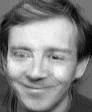
\includegraphics[width=0.25\textwidth]{PartialReconstruction4.jpg} & 5. 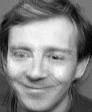
\includegraphics[width=0.25\textwidth]{PartialReconstruction5.jpg} \\
    6. 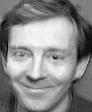
\includegraphics[width=0.25\textwidth]{PartialReconstruction6.jpg} & 7. 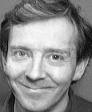
\includegraphics[width=0.25\textwidth]{PartialReconstruction7.jpg} & 8. 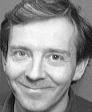
\includegraphics[width=0.25\textwidth]{PartialReconstruction8.jpg} \\
    9. 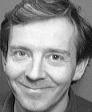
\includegraphics[width=0.25\textwidth]{PartialReconstruction9.jpg} & 10. 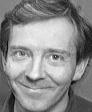
\includegraphics[width=0.25\textwidth]{PartialReconstruction10.jpg}
  \end{tabular}
\end{figure}

\FloatBarrier
\section{Partial Reconstructions from 4.6}
\begin{figure}[h!]
  \caption{Images of all 6 partial reconstructions, including mean}
  \centering
  
  \begin{tabular}{ c c c }
    0. 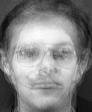
\includegraphics[width=0.25\textwidth]{Final/PartialReconstruction0.jpg} & 1. 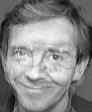
\includegraphics[width=0.25\textwidth]{Final/PartialReconstruction1.jpg} & 2. 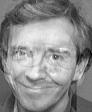
\includegraphics[width=0.25\textwidth]{Final/PartialReconstruction2.jpg} \\
    3. 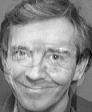
\includegraphics[width=0.25\textwidth]{Final/PartialReconstruction3.jpg} & 4. 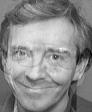
\includegraphics[width=0.25\textwidth]{Final/PartialReconstruction4.jpg} & 5. 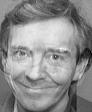
\includegraphics[width=0.25\textwidth]{Final/PartialReconstruction5.jpg} \\
    6. 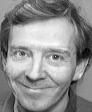
\includegraphics[width=0.25\textwidth]{Final/PartialReconstruction6.jpg}
  \end{tabular}
\end{figure}

\end{document}